\section{Cageon confinement}\label{sec:cageon-confinement}

Cageon confinement evaluates the even outer confinement cages after the field, shell, and cage structures have been declared. Naming conventions and count compression are fixed in \apref{app:curling-curls}; this section evaluates confinement by PADAR burden, shedding, TTL, and the \(\Qfour\) audit.

\subsection{Even forms}\label{subsec:cageon-even-forms}
The even sequence separates the current-side double form, the inner cage, and the outer cageons:
\[
E_2=\mathrm{duon},
\qquad
E_2^{0}=\text{open-seat duon},
\qquad
E_2^{\pm}=\mathrm{duad}.
\]
Duon is two dion returns through a monon hinge:
\[
\mathrm{duon}=D_i\mu D_j,
\qquad
\mu\in\{-1,0,+1\}.
\]
The value \(\mu=0\) is the open-seat duon, while \(\mu=\pm1\) is the seat-closed duon, i.e. the duad. Thus duon is \(E_2\); duad is the seated state of \(E_2\).

The inner four-seat cage is
\[
E_4=\mathrm{tetron}.
\]
Tetron is the default inner cage with four seats. Hexon, octon, and decon organize the outer shell paths.

\subsection{Outer cageons}\label{subsec:outer-cageons}
A cageon is an outer even confinement cage. Write
\[
\mathsf C_{2m}=\text{cageon of order }2m,
\qquad m\ge3.
\]
The named outer cageons are
\[
\mathsf C_6=\mathrm{hexon},
\qquad
\mathsf C_8=\mathrm{octon},
\qquad
\mathsf C_{10}=\mathrm{decon}.
\]
Higher cageons are written \(\mathsf C_{12},\mathsf C_{14},\mathsf C_{16},\ldots\) until spoken names are declared.

Hexon is the first outer cageon because the hinge triad supplies left/right threefold closure:
\[
\mathsf H_3+\mathsf H_3=6.
\]
Equivalently,
\[
3+3=6.
\]

\subsection{Shared cage compression}\label{subsec:shared-cage-compression}
Use the compact count basis
\[
\mathcal B_{\mathrm{curl}}=(3:3,
3:4,
1:2)=(\mathrm{Tritrio},\mathrm{Tetratrio},\mathrm{Dimon}).
\]
A count form
\[
a:b:c::L
\]
means
\[
\mathrm{Tritrio}^{a}::\mathrm{Tetratrio}^{b}::\mathrm{Dimon}^{c}::\operatorname{out}(L).
\]
The basic shared hexon is
\[
1:1:0::6
=
\mathrm{Tritrio}::\mathrm{Tetratrio}::\mathrm{hexon}.
\]
The equivalent expanded numeric form is
\[
(3:3)^1::(3:4)^1::(1:2)^0::6.
\]

\subsection{Filled shared cageons}\label{subsec:filled-shared-cageons}
A filled shared cageon has
\[
m:m:0::2m,
\qquad
m\ge3.
\]
Examples are
\[
3:3:0::6
=
\mathrm{Tritrio}^{3}::\mathrm{Tetratrio}^{3}::\mathrm{hexon},
\]
\[
4:4:0::8
=
\mathrm{Tritrio}^{4}::\mathrm{Tetratrio}^{4}::\mathrm{octon},
\]
\[
5:5:0::10
=
\mathrm{Tritrio}^{5}::\mathrm{Tetratrio}^{5}::\mathrm{decon}.
\]
The confinement ratio is
\[
\#(3:3):\#(3:4)=1:1.
\]

\subsection{Coord-0 cageon grouping}\label{subsec:coord-zero-cageon-grouping}
At coordinate \(0\), write element-facing cageon declarations as
\[
0\mid-::Z:A:0:L\langle a:b:c::L\rangle.
\]
For filled cageon grouping,
\[
0\mid-::Z:A:0:2m\langle m:m:0::2m\rangle.
\]
Define the cumulative group boundary
\[
B_m=\sum_{k=3}^{m}2k=m(m+1)-6,
\qquad
B_2=0.
\]
Then
\[
B_{m-1}<Z\le B_m
\]
selects the coord-0 cageon group.

\begin{center}
\begin{tabular}{ccc}
\toprule
Group & Cageon & Filled form\\
\midrule
\(G_3\) & \(\mathsf C_6\) / hexon & \(3:3:0::6\)\\
\(G_4\) & \(\mathsf C_8\) / octon & \(4:4:0::8\)\\
\(G_5\) & \(\mathsf C_{10}\) / decon & \(5:5:0::10\)\\
\(G_6\) & \(\mathsf C_{12}\) & \(6:6:0::12\)\\
\(G_7\) & \(\mathsf C_{14}\) & \(7:7:0::14\)\\
\bottomrule
\end{tabular}
\end{center}
For example, \(Z=26\) falls in
\[
G_6,
\qquad
\mathsf C_{12},
\qquad
6:6:0::12.
\]

\subsection{TTL condition}\label{subsec:cageon-ttl-condition}
For a cageon declaration \(\mathcal C=a:b:c::L\), write
\[
\mathrm{TTL}_{\mathcal C}(\partial F,\omega)
\]
for the retained tick duration before PADAR closure failure. Retention on the declared window is
\[
\mathrm{TTL}_{\mathcal C}(\partial F,\omega)\ge |\omega|.
\]
If
\[
\mathrm{TTL}_{\mathcal C}(\partial F,\omega)<|\omega|,
\]
the path sheds, re-enters, or decays before the window closes.

\begin{figure}[H]
\centering
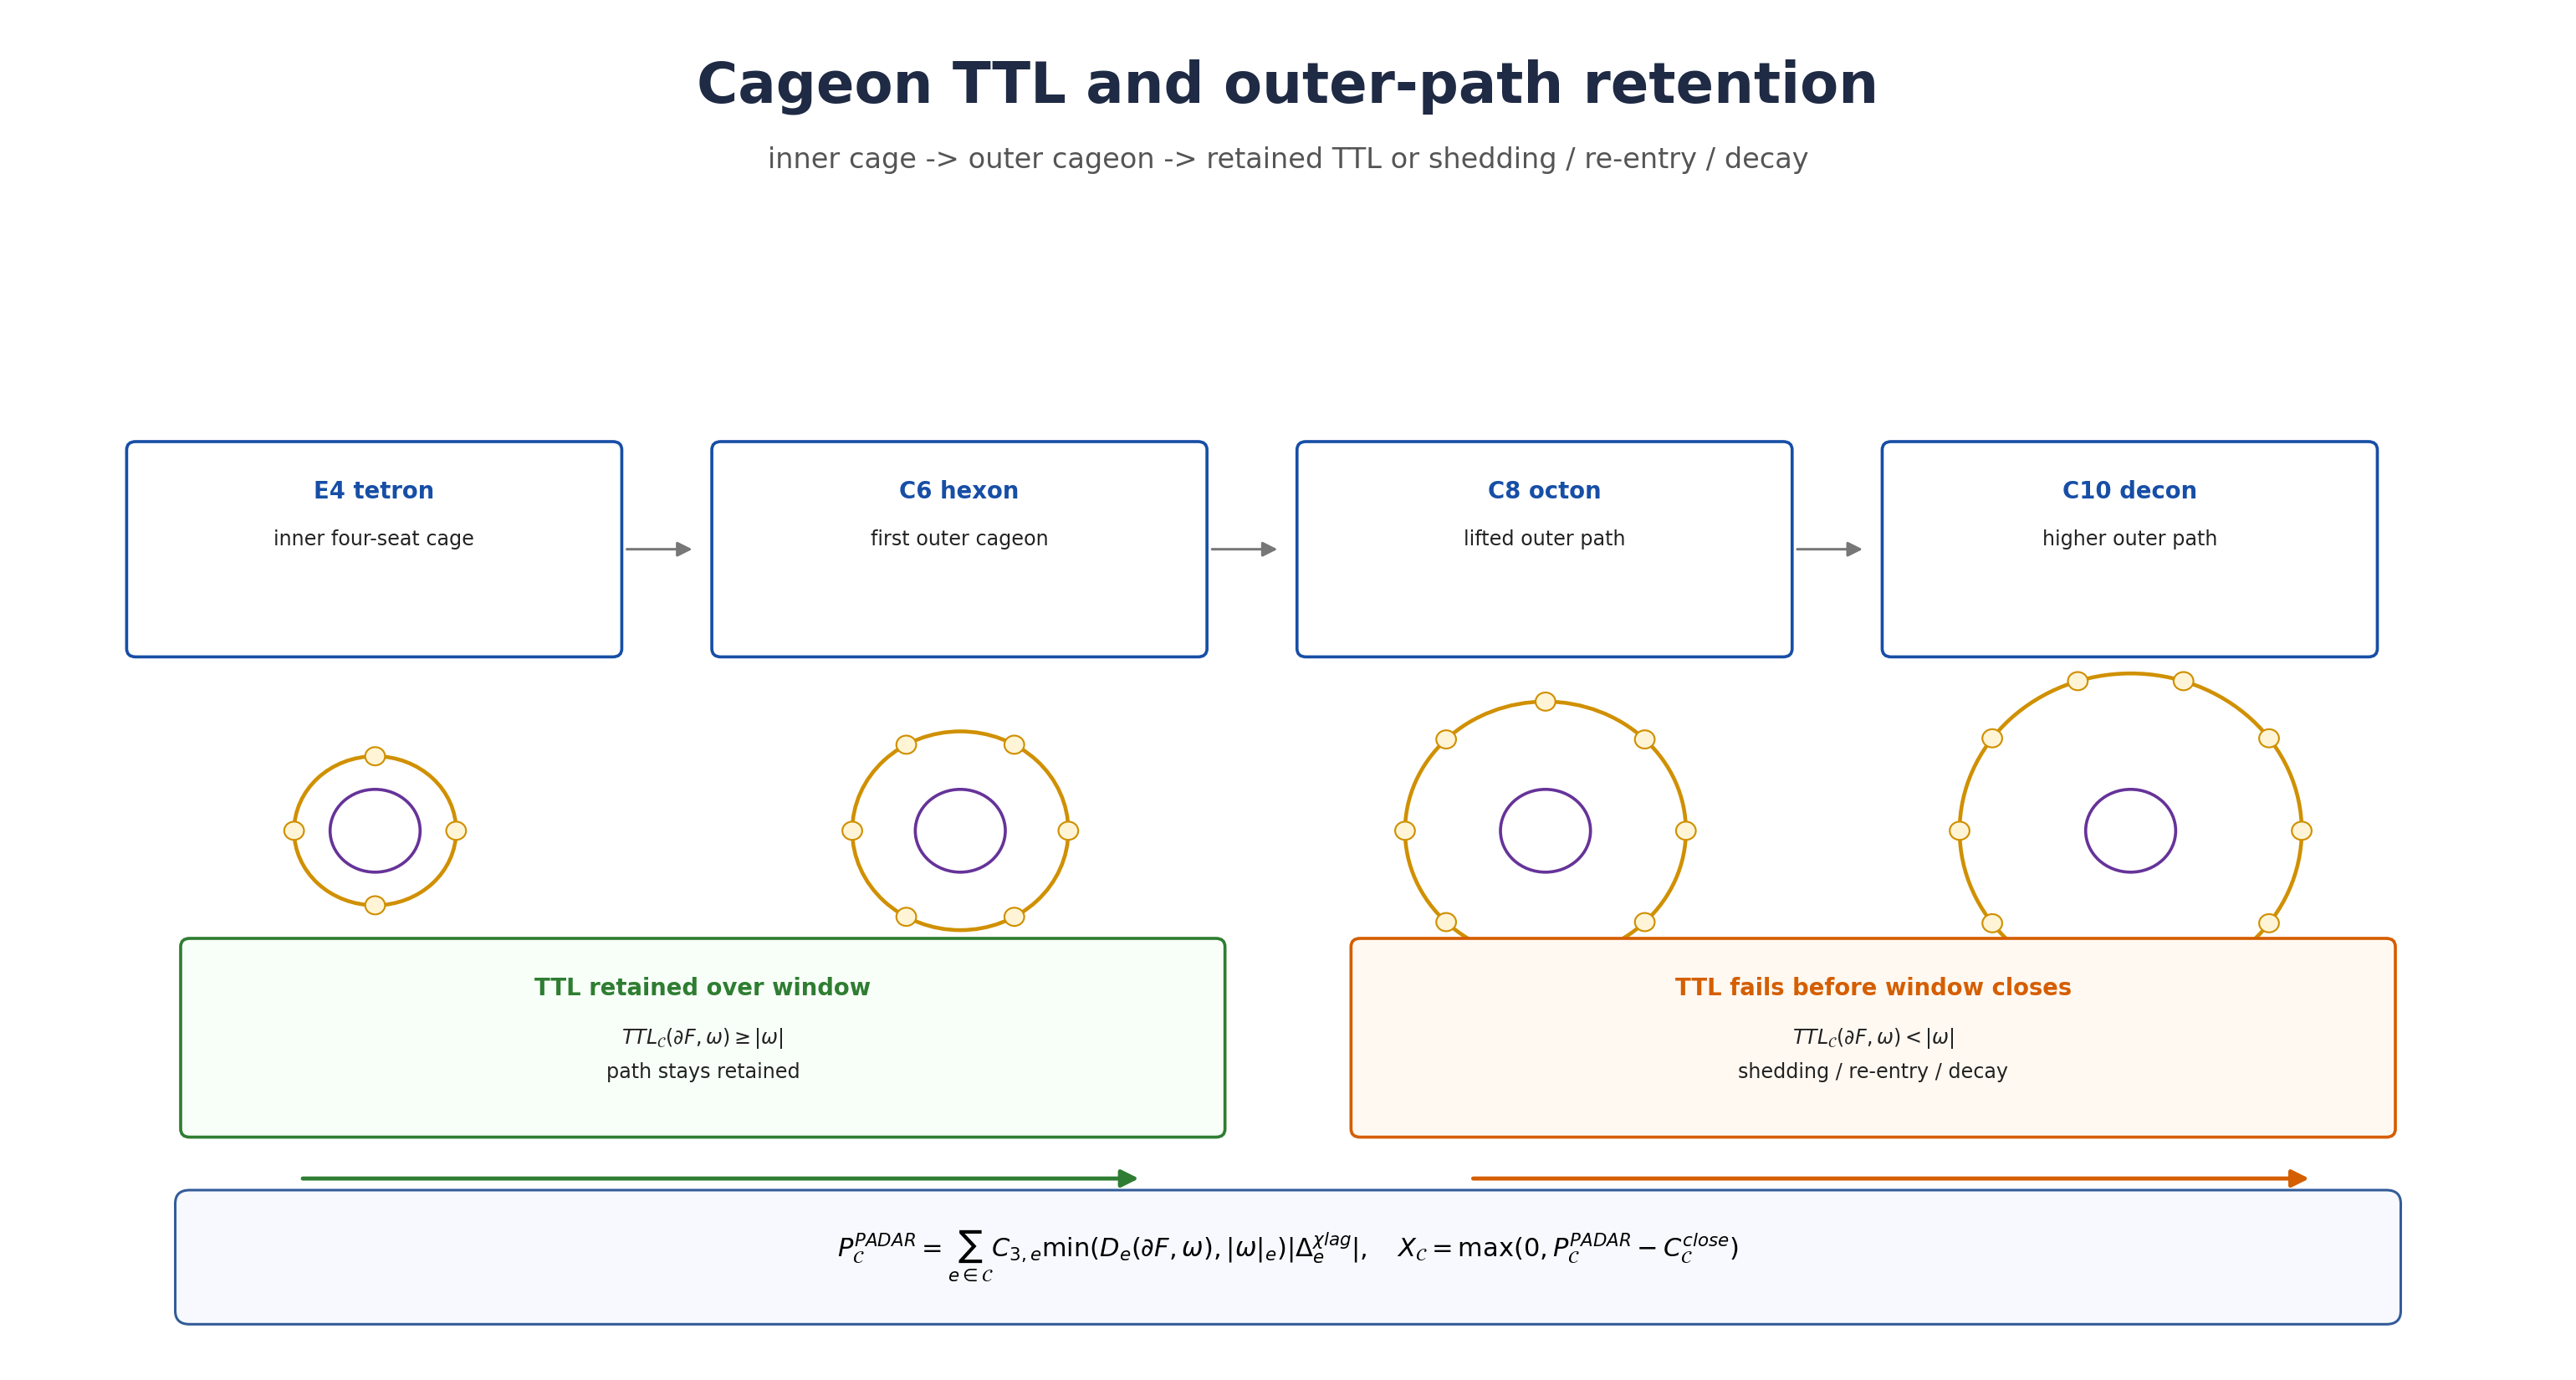
\includegraphics[width=0.98\linewidth]{figures_jpg/v39_17_cageon_ttl_outer_path_retention.png}
\caption{Cageon TTL and outer-path retention. Tetron is the inner four-seat cage; hexon, octon, and decon are outer cageon paths. Retained TTL keeps the path on the declared window; TTL failure produces shedding, re-entry, or decay.}
\label{fig:v39-cageon-ttl-outer-path-retention}
\end{figure}

\subsection{PADAR closure for cageons}\label{subsec:cageon-padar-closure}
Cageon confinement is evaluated by PADAR closure on a declared boundary/window. For a cageon declaration \(\mathcal C=a:b:c::L\), define
\[
P_{\mathcal C}^{\PADAR}(\partial F,\omega)
=
\sum_{e\in\mathcal C}
C_{3,e}
\min\!\left(D_e(\partial F,\omega),|\omega|_e\right)
\left|\Delta^{\chi\mathrm{lag}}_e\right|.
\]
The closure excess is
\[
X_{\mathcal C}(\partial F,\omega)
=
\max\!\left(
0,
P_{\mathcal C}^{\PADAR}(\partial F,\omega)
-
C_{\mathcal C}^{\mathrm{close}}(\partial F,\omega)
\right).
\]
The value and placement of \(X_{\mathcal C}\) determine local reclosure, exoshedding, endoshedding, or transmutation routing.

\paragraph{Exoshedding.}
Exoshedding is closure excess crossing the outer cage boundary.

\paragraph{Endoshedding.}
Endoshedding is closure excess retained through an inner reclosure path.

\paragraph{Transmutation routing.}
Transmutation routing is closure excess redirected into a different retained cageon or shell path after PADAR closure changes.

The core diagnostics are
\[
D_e\leftrightarrow R^{\mathrm{asym}}_e,
\qquad
P_{\mathcal C}^{\PADAR},
\qquad
X_{\mathcal C},
\qquad
\mathrm{TTL}_{\mathcal C},
\qquad
\Qfour\text{ audit}.
\]

\subsection{Confinement patterns}\label{subsec:cageon-confinement-patterns}
Current confinement patterns are
\[
3:3:6\parallel3:4:6
\rightarrow
3:3::3:4::6
\rightarrow
1:1:0::6.
\]
Filled hexon confinement is
\[
3:3:0::6
=
\mathrm{Tritrio}^{3}::\mathrm{Tetratrio}^{3}::\mathrm{hexon}.
\]
The upward cage lift is
\[
3:3:0::6
\rightarrow
4:4:0::8
\rightarrow
5:5:0::10,
\]
namely
\[
\mathrm{Tritrio}^{3}::\mathrm{Tetratrio}^{3}::\mathrm{hexon}
\rightarrow
\mathrm{Tritrio}^{4}::\mathrm{Tetratrio}^{4}::\mathrm{octon}
\rightarrow
\mathrm{Tritrio}^{5}::\mathrm{Tetratrio}^{5}::\mathrm{decon}.
\]
The hexon fills, then octon becomes the next confinement cageon.
